\section{可在内核态和用户态之间进行切换的ucore}\label{ux53efux5728ux5185ux6838ux6001ux548cux7528ux6237ux6001ux4e4bux95f4ux8fdbux884cux5207ux6362ux7684ucore}

在操作系统原理中,一直强调操作系统运行在内核态(特权态),应用程序运行在用户态(非特权态)。但为什么说处于用户态的应用程序就不能访问内核态的数据,而内核态的操作系统可以访问用户态的数据?我们有没有一个project来体验内核态和用户态的区别是什么?更进一步体验如何在内核态和用户态之间进行切换呢?project4.1.1为此进行了尝试。

\subsection{实验目标}\label{ux5b9eux9a8cux76eeux6807}

通过学习和实践,读者可以了解如何CPU处不同特权态下的执行特点和限制,理解如何从内核态切换到用户态,以及如何从用户态切换到内核态。

\subsection{proj4.1.1概述}\label{proj4.1.1ux6982ux8ff0}

\subsubsection{实现描述}\label{ux5b9eux73b0ux63cfux8ff0}

proj4.1.1建立在proj4.1(当然是基于proj4)基础之上,主要完成了用户态(非特权态)与内核态相互切换的过程。相对于proj4,主要增加了两部分工作,一部分是从用户态返回内核态的准备工作,即建立任务段(Task
Segment)和任务段描述符(SEG\_TSS),设置陷阱中断号(T\_SWITCH\_TOK)和对应的中断处理例程。另外一部分是对内核栈进行各种特殊处理,使得能够完成内核态切换到用户态或用户态切换到内核态的工作。

\subsubsection{项目组成}\label{ux9879ux76eeux7ec4ux6210}

这里我们通过proj4.1.1来完成此事。proj4.1.1整体目录结构如下所示:

\begin{lstlisting}
proj4.1.1
|-- kern
|   |-- init
|   |   `-- init.c
|   |-- mm
|   |   |-- memlayout.h
|   |   |-- mmu.h
|   |   |-- pmm.c
|   |   `-- pmm.h
|   `-- trap
|       |-- trap.c
|       |-- trapentry.S
|       |-- trap.h
|       `-- vectors.S
……
\end{lstlisting}

相对于proj4,改动不多,主要修改和增加的文件如下:

\begin{itemize}
\item
  memlayout.h:定义了全局描述符的索引值和一些段描述符的属性。
\item
  pmm.{[}ch{]}:为了能够使CPU从用户态转换到内核态,在ucore初始化时,设置任务段和任务段描述符,重新加载任务段和段描述符表;
\item
  trap.c:设置自定义的陷阱中断T\_SWITCH\_TOK(用于用户态切换到内核态)和实现对自定义的陷阱中断T\_SWITCH\_TOK/T\_SWITCH\_TOU的中断处理例程,使得CPU能够在内核态和用户态之间切换。
\end{itemize}

\subsubsection{编译运行}\label{ux7f16ux8bd1ux8fd0ux884c}

编译并运行proj4.1.1的命令如下:

\begin{lstlisting}
make
make qemu
\end{lstlisting}

则可以得到如下显示界面

\begin{figure}[htbp]
\centering
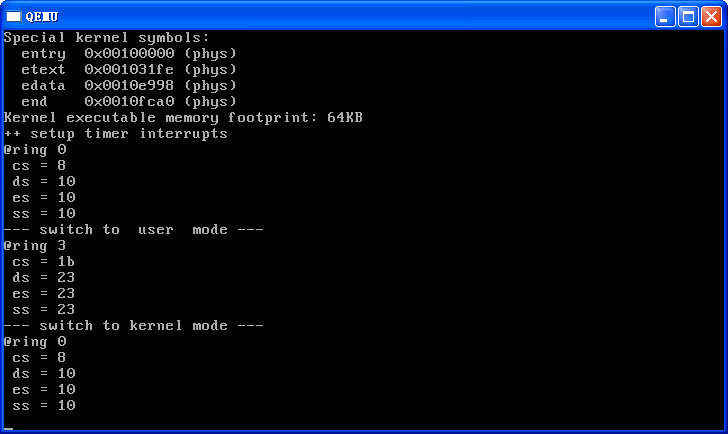
\includegraphics{figures/3.5.2.1.png}
\caption{3.5.2.1}
\end{figure}

通过上图,我们可以看到ucore在切换到用户态之前,先显示了当前CPU的特权级(CS的最低两位),CS/DS/ES/SS的值(即对应的段描述符表的索引值),可以看到特权级为0。根据lgdt函数(位于kern/mm/pmm.c中)的处理,CS的值是内核代码段描述符的索引下标,DS/ES/SS的值是内核数据段描述符的索引下标;而在切换到用户态后,又显示了一下,当前CPU的特权级为3,
CS的值为1b,DS/ES/SS的值为23,把这四个寄存器的值\&0xfc,则分别为0x18(SEG\_UTEXT)和0x20(SEG\_UDATA),说明确实运行在用户态了。在执行了系统调用T\_SWITCH\_TOK后,又回到了内核态。下面我们将分析到底发生了什么事情。
